\documentclass[10pt,twocolumn]{article}
\usepackage[letterpaper,margin=0.75in]{geometry}
\usepackage[T1]{fontenc}
\usepackage{times}
\renewcommand{\ttdefault}{lmtt}
\usepackage{graphicx}
\usepackage{booktabs}
\usepackage{amsmath}
\usepackage{xcolor}
\usepackage[hidelinks]{hyperref}
\usepackage{natbib}
\setcitestyle{numbers,square}
\setlength{\bibsep}{1pt}
\setlength{\columnsep}{0.25in}
\makeatletter
\renewcommand\section{\@startsection{section}{1}{\z@}{-1.5ex plus -.4ex minus -.2ex}{0.7ex plus .2ex}{\normalfont\large\bfseries\raggedright}}
\renewcommand\subsection{\@startsection{subsection}{2}{\z@}{-1.1ex plus -.3ex minus -.2ex}{0.4ex plus .1ex}{\normalfont\normalsize\bfseries\raggedright}}
\renewcommand{\@makecaption}[2]{\vskip\abovecaptionskip{\small\textbf{#1.} #2\par}\vskip\belowcaptionskip}
\makeatother
\setlength{\parskip}{0pt}
\setlength{\textfloatsep}{8pt plus 2pt minus 2pt}
\setlength{\floatsep}{6pt}
\setlength{\dbltextfloatsep}{8pt plus 2pt minus 2pt}
\setlength{\dblfloatsep}{6pt}
\AtBeginDocument{\setlength{\abovedisplayskip}{3pt plus 1pt}\setlength{\belowdisplayskip}{3pt plus 1pt}%
\setlength{\abovedisplayshortskip}{1pt}\setlength{\belowdisplayshortskip}{2pt plus 1pt}}
\setlength{\abovecaptionskip}{2pt}
\newcommand{\code}[1]{\texttt{\small #1}}
% Generated by analysis/report_numbers.py from results/summary/*.json. Do not edit.
\newcommand{\Model}{claude-haiku-5-5}
\newcommand{\CliVersion}{2.1.330}
\newcommand{\NCalls}{2{,}582}
\newcommand{\TotalCost}{3.16}
\newcommand{\TotalTokensM}{8.1}
\newcommand{\NTests}{296}
\newcommand{\VibeWords}{28}
\newcommand{\SpecWords}{114}
\newcommand{\VibeN}{300}
\newcommand{\VibePass}{231}
\newcommand{\VibeNM}{58}
\newcommand{\VibeFail}{11}
\newcommand{\VibePassRate}{77\%}
\newcommand{\VibePassLo}{72\%}
\newcommand{\VibePassHi}{81\%}
\newcommand{\NmGivenFail}{84\%}
\newcommand{\NmGivenFailLo}{65\%}
\newcommand{\NmGivenFailHi}{98\%}
\newcommand{\MeanEntropy}{0.24}
\newcommand{\MeanVar}{0.056}
\newcommand{\NStochastic}{9}
\newcommand{\NAlwaysPass}{18}
\newcommand{\NNeverPass}{3}
\newcommand{\NWithNM}{11}
\newcommand{\MeanFracFailures}{83\%}
\newcommand{\MedianFracFailures}{90\%}
\newcommand{\DistinctBehaviours}{1.43}
\newcommand{\CodeSimilarity}{0.50}
\newcommand{\StochEntropy}{0.80}
\newcommand{\PassHumaneval}{85\%}
\newcommand{\StochHumaneval}{4}
\newcommand{\PassMbpp}{68\%}
\newcommand{\StochMbpp}{1}
\newcommand{\PassOriginal}{78\%}
\newcommand{\StochOriginal}{4}
\newcommand{\BlindHazOne}{77\%}
\newcommand{\BlindCumOne}{77\%}
\newcommand{\BlindHazTwo}{24\%}
\newcommand{\BlindCumTwo}{83\%}
\newcommand{\BlindHazThree}{14\%}
\newcommand{\BlindCumThree}{85\%}
\newcommand{\BlindHazFour}{9\%}
\newcommand{\BlindCumFour}{87\%}
\newcommand{\BlindHazFive}{7\%}
\newcommand{\BlindCumFive}{87\%}
\newcommand{\BlindHazTwoLo}{11\%}
\newcommand{\BlindHazTwoHi}{43\%}
\newcommand{\EpReachedOne}{300}
\newcommand{\EpHazOne}{77\%}
\newcommand{\EpCumOne}{77\%}
\newcommand{\EpReachedTwo}{69}
\newcommand{\EpHazTwo}{91\%}
\newcommand{\EpCumTwo}{98\%}
\newcommand{\EpReachedThree}{6}
\newcommand{\EpHazThree}{100\%}
\newcommand{\EpCumThree}{100\%}
\newcommand{\EpReachedFour}{0}
\newcommand{\EpCumFour}{100\%}
\newcommand{\EpReachedFive}{0}
\newcommand{\EpCumFive}{100\%}
\newcommand{\PassAfterNM}{94\%}
\newcommand{\NAfterNM}{63}
\newcommand{\PassAfterFail}{83\%}
\newcommand{\NAfterFail}{12}
\newcommand{\RegressionRate}{0\%}
\newcommand{\ConsecSimilarity}{0.83}
\newcommand{\EpMeanTurns}{1.25}
\newcommand{\EpFinalPass}{100\%}
\newcommand{\KStar}{3}
\newcommand{\SpecPassRate}{100\%}
\newcommand{\SpecN}{300}
\newcommand{\SpecEntropy}{0.00}
\newcommand{\ModalSignatureShare}{87\%}
\newcommand{\NFailedPulls}{69}
\newcommand{\PTwoPass}{100\%}
\newcommand{\PTwoPassLo}{100\%}
\newcommand{\PTwoPassHi}{100\%}
\newcommand{\PTwoModelPass}{100\%}
\newcommand{\PTwoN}{300}
\newcommand{\PTwoVisH}{0.16}
\newcommand{\PTwoNM}{0.11}
\newcommand{\PTwoRetries}{0.11}
\newcommand{\PTwoDecisions}{0.00}
\newcommand{\PTwoReview}{0.57}
\newcommand{\PTwoHumanFrac}{0\%}
\newcommand{\PTwoCalls}{5.6}
\newcommand{\PTwoTokK}{12.0}
\newcommand{\PTwoLat}{7.2}
\newcommand{\PTwoHandoffs}{0}
\newcommand{\PTwoEngaged}{0}
\newcommand{\PTwoPassHumaneval}{100\%}
\newcommand{\PTwoPassMbpp}{100\%}
\newcommand{\PTwoPassOriginal}{100\%}
\newcommand{\PTwoVisHRed}{59\%}
\newcommand{\PTwoNMRed}{49\%}
\newcommand{\PTwoRetryRed}{55\%}
\newcommand{\PTwoTokX}{4.1}
\newcommand{\POnePass}{100\%}
\newcommand{\POnePassLo}{100\%}
\newcommand{\POnePassHi}{100\%}
\newcommand{\POneModelPass}{100\%}
\newcommand{\POneN}{300}
\newcommand{\POneVisH}{0.38}
\newcommand{\POneNM}{0.21}
\newcommand{\POneRetries}{0.25}
\newcommand{\POneDecisions}{0.00}
\newcommand{\POneReview}{0.00}
\newcommand{\POneHumanFrac}{0\%}
\newcommand{\POneCalls}{1.2}
\newcommand{\POneTokK}{2.9}
\newcommand{\POneLat}{7.0}
\newcommand{\POneHandoffs}{0}
\newcommand{\POneEngaged}{0}
\newcommand{\POnePassHumaneval}{100\%}
\newcommand{\POnePassMbpp}{100\%}
\newcommand{\POnePassOriginal}{100\%}
\newcommand{\POneVisHRed}{-0\%}
\newcommand{\POneNMRed}{-0\%}
\newcommand{\POneRetryRed}{-0\%}
\newcommand{\POneTokX}{1.0}
\newcommand{\POneKOnePass}{98\%}
\newcommand{\POneKOnePassLo}{95\%}
\newcommand{\POneKOnePassHi}{100\%}
\newcommand{\POneKOneModelPass}{77\%}
\newcommand{\POneKOneN}{300}
\newcommand{\POneKOneVisH}{0.29}
\newcommand{\POneKOneNM}{0.19}
\newcommand{\POneKOneRetries}{0.00}
\newcommand{\POneKOneDecisions}{0.41}
\newcommand{\POneKOneReview}{0.00}
\newcommand{\POneKOneHumanFrac}{7\%}
\newcommand{\POneKOneCalls}{1.2}
\newcommand{\POneKOneTokK}{3.3}
\newcommand{\POneKOneLat}{8.8}
\newcommand{\POneKOneHandoffs}{69}
\newcommand{\POneKOneRescue}{91\%}
\newcommand{\POneKOneHumanFracEngaged}{29\%}
\newcommand{\POneKOneEngaged}{69}
\newcommand{\POneKOneSoundness}{93\%}
\newcommand{\POneKOneInvTotal}{522}
\newcommand{\POneKOneCompliance}{100\%}
\newcommand{\POneKOneHoles}{1.8}
\newcommand{\POneKOnePassHumaneval}{100\%}
\newcommand{\POneKOnePassMbpp}{99\%}
\newcommand{\POneKOnePassOriginal}{95\%}
\newcommand{\POneKOneVisHRed}{23\%}
\newcommand{\POneKOneNMRed}{8\%}
\newcommand{\POneKOneRetryRed}{100\%}
\newcommand{\POneKOneTokX}{1.2}
\newcommand{\POneKTwoPass}{99\%}
\newcommand{\POneKTwoPassLo}{98\%}
\newcommand{\POneKTwoPassHi}{100\%}
\newcommand{\POneKTwoModelPass}{98\%}
\newcommand{\POneKTwoN}{300}
\newcommand{\POneKTwoVisH}{0.39}
\newcommand{\POneKTwoNM}{0.21}
\newcommand{\POneKTwoRetries}{0.23}
\newcommand{\POneKTwoDecisions}{0.05}
\newcommand{\POneKTwoReview}{0.00}
\newcommand{\POneKTwoHumanFrac}{1\%}
\newcommand{\POneKTwoCalls}{1.2}
\newcommand{\POneKTwoTokK}{2.9}
\newcommand{\POneKTwoLat}{7.1}
\newcommand{\POneKTwoHandoffs}{6}
\newcommand{\POneKTwoRescue}{67\%}
\newcommand{\POneKTwoHumanFracEngaged}{26\%}
\newcommand{\POneKTwoEngaged}{6}
\newcommand{\POneKTwoSoundness}{92\%}
\newcommand{\POneKTwoInvTotal}{36}
\newcommand{\POneKTwoCompliance}{100\%}
\newcommand{\POneKTwoHoles}{2.3}
\newcommand{\POneKTwoPassHumaneval}{100\%}
\newcommand{\POneKTwoPassMbpp}{100\%}
\newcommand{\POneKTwoPassOriginal}{98\%}
\newcommand{\POneKTwoVisHRed}{-1\%}
\newcommand{\POneKTwoNMRed}{-0\%}
\newcommand{\POneKTwoRetryRed}{8\%}
\newcommand{\POneKTwoTokX}{1.0}
\newcommand{\BasePass}{100\%}
\newcommand{\BasePassLo}{100\%}
\newcommand{\BasePassHi}{100\%}
\newcommand{\BaseModelPass}{100\%}
\newcommand{\BaseN}{300}
\newcommand{\BaseVisH}{0.38}
\newcommand{\BaseNM}{0.21}
\newcommand{\BaseRetries}{0.25}
\newcommand{\BaseDecisions}{0.00}
\newcommand{\BaseReview}{0.00}
\newcommand{\BaseHumanFrac}{0\%}
\newcommand{\BaseCalls}{1.2}
\newcommand{\BaseTokK}{2.9}
\newcommand{\BaseLat}{7.0}
\newcommand{\BaseHandoffs}{0}
\newcommand{\BaseEngaged}{0}
\newcommand{\BasePassHumaneval}{100\%}
\newcommand{\BasePassMbpp}{100\%}
\newcommand{\BasePassOriginal}{100\%}
\newcommand{\BaseVisHRed}{-0\%}
\newcommand{\BaseNMRed}{-0\%}
\newcommand{\BaseRetryRed}{-0\%}
\newcommand{\BaseTokX}{1.0}
\newcommand{\PThreePass}{99\%}
\newcommand{\PThreePassLo}{98\%}
\newcommand{\PThreePassHi}{100\%}
\newcommand{\PThreeModelPass}{99\%}
\newcommand{\PThreeN}{300}
\newcommand{\PThreeVisH}{0.34}
\newcommand{\PThreeNM}{0.00}
\newcommand{\PThreeRetries}{0.00}
\newcommand{\PThreeDecisions}{0.30}
\newcommand{\PThreeReview}{0.30}
\newcommand{\PThreeHumanFrac}{0\%}
\newcommand{\PThreeCalls}{1.6}
\newcommand{\PThreeTokK}{3.6}
\newcommand{\PThreeLat}{8.7}
\newcommand{\PThreeHandoffs}{0}
\newcommand{\PThreeHumanFracEngaged}{0\%}
\newcommand{\PThreeEngaged}{69}
\newcommand{\PThreeCodeFree}{80\%}
\newcommand{\PThreeNHints}{91}
\newcommand{\PThreePassHumaneval}{100\%}
\newcommand{\PThreePassMbpp}{100\%}
\newcommand{\PThreePassOriginal}{98\%}
\newcommand{\PThreeVisHRed}{10\%}
\newcommand{\PThreeNMRed}{100\%}
\newcommand{\PThreeRetryRed}{100\%}
\newcommand{\PThreeTokX}{1.2}
\newcommand{\PFourPass}{85\%}
\newcommand{\PFourPassLo}{74\%}
\newcommand{\PFourPassHi}{93\%}
\newcommand{\PFourModelPass}{0\%}
\newcommand{\PFourN}{150}
\newcommand{\PFourVisH}{0.00}
\newcommand{\PFourNM}{0.00}
\newcommand{\PFourRetries}{0.00}
\newcommand{\PFourDecisions}{2.19}
\newcommand{\PFourReview}{0.00}
\newcommand{\PFourHumanFrac}{31\%}
\newcommand{\PFourCalls}{1.0}
\newcommand{\PFourTokK}{4.8}
\newcommand{\PFourLat}{14.9}
\newcommand{\PFourHandoffs}{0}
\newcommand{\PFourHumanFracEngaged}{31\%}
\newcommand{\PFourEngaged}{150}
\newcommand{\PFourSoundness}{92\%}
\newcommand{\PFourInvTotal}{1133}
\newcommand{\PFourCompliance}{100\%}
\newcommand{\PFourHoles}{2.2}
\newcommand{\PFourPassHumaneval}{98\%}
\newcommand{\PFourPassMbpp}{86\%}
\newcommand{\PFourPassOriginal}{70\%}
\newcommand{\PFourVisHRed}{100\%}
\newcommand{\PFourNMRed}{100\%}
\newcommand{\PFourRetryRed}{100\%}
\newcommand{\PFourTokX}{1.6}
\newcommand{\PFourFailures}{23}
\newcommand{\PFourSingleFail}{17}
\newcommand{\NContested}{12}
\newcommand{\PTwoContestedPass}{100\%}
\newcommand{\PTwoContestedNM}{0.27}
\newcommand{\PTwoContestedDecisions}{0.00}
\newcommand{\POneContestedPass}{100\%}
\newcommand{\POneContestedNM}{0.53}
\newcommand{\POneContestedDecisions}{0.00}
\newcommand{\POneKOneContestedPass}{95\%}
\newcommand{\POneKOneContestedNM}{0.48}
\newcommand{\POneKOneContestedDecisions}{1.02}
\newcommand{\POneKTwoContestedPass}{98\%}
\newcommand{\POneKTwoContestedNM}{0.53}
\newcommand{\POneKTwoContestedDecisions}{0.12}
\newcommand{\BaseContestedPass}{100\%}
\newcommand{\BaseContestedNM}{0.53}
\newcommand{\BaseContestedDecisions}{0.00}
\newcommand{\PThreeContestedPass}{98\%}
\newcommand{\PThreeContestedNM}{0.00}
\newcommand{\PThreeContestedDecisions}{0.74}
\newcommand{\PFourContestedPass}{80\%}
\newcommand{\PFourContestedNM}{0.00}
\newcommand{\PFourContestedDecisions}{2.20}
\newcommand{\NVisible}{3}
\newcommand{\NHeldOut}{206}
\newcommand{\RVibePass}{78\%}
\newcommand{\RVibePassLo}{65\%}
\newcommand{\RVibePassHi}{90\%}
\newcommand{\RVibeN}{300}
\newcommand{\RVibeVisPass}{100\%}
\newcommand{\RVibeSilent}{22\%}
\newcommand{\RVibeSilentGivenVis}{22\%}
\newcommand{\RVibeNM}{0.01}
\newcommand{\RVibeDecisions}{0.00}
\newcommand{\RVibeTurns}{0.03}
\newcommand{\RVibeShown}{35}
\newcommand{\RVibeHumanFrac}{0\%}
\newcommand{\RVibeCalls}{1.0}
\newcommand{\RVibeTokK}{2.2}
\newcommand{\RVibeTokX}{1.0}
\newcommand{\RVibeLat}{5.7}
\newcommand{\RVibeClar}{0.00}
\newcommand{\RVibeContestedPass}{46\%}
\newcommand{\RVibeContestedSilent}{54\%}
\newcommand{\RVibeDelta}{0}
\newcommand{\RVibeDeltaLo}{0}
\newcommand{\RVibeDeltaHi}{0}
\newcommand{\RVibeContestedDelta}{0}
\newcommand{\RVibeContestedDeltaLo}{0}
\newcommand{\RVibeContestedDeltaHi}{0}
\newcommand{\RVibeSilentDelta}{0}
\newcommand{\RVibeSilentDeltaLo}{0}
\newcommand{\RVibeSilentDeltaHi}{0}
\newcommand{\RVibePassHumaneval}{89\%}
\newcommand{\RVibePassMbpp}{68\%}
\newcommand{\RVibePassOriginal}{78\%}
\newcommand{\RAttPass}{100\%}
\newcommand{\RAttPassLo}{100\%}
\newcommand{\RAttPassHi}{100\%}
\newcommand{\RAttN}{300}
\newcommand{\RAttVisPass}{100\%}
\newcommand{\RAttSilent}{0\%}
\newcommand{\RAttSilentGivenVis}{0\%}
\newcommand{\RAttNM}{0.01}
\newcommand{\RAttDecisions}{0.56}
\newcommand{\RAttTurns}{1.56}
\newcommand{\RAttShown}{57}
\newcommand{\RAttHumanFrac}{0\%}
\newcommand{\RAttCalls}{1.6}
\newcommand{\RAttTokK}{3.7}
\newcommand{\RAttTokX}{1.7}
\newcommand{\RAttLat}{8.0}
\newcommand{\RAttClar}{0.56}
\newcommand{\RAttContestedPass}{100\%}
\newcommand{\RAttContestedSilent}{0\%}
\newcommand{\RAttDelta}{$+$22}
\newcommand{\RAttDeltaLo}{$+$10}
\newcommand{\RAttDeltaHi}{$+$35}
\newcommand{\RAttContestedDelta}{$+$54}
\newcommand{\RAttContestedDeltaLo}{$+$34}
\newcommand{\RAttContestedDeltaHi}{$+$74}
\newcommand{\RAttSilentDelta}{$-$22}
\newcommand{\RAttSilentDeltaLo}{$-$35}
\newcommand{\RAttSilentDeltaHi}{$-$10}
\newcommand{\RAttPassHumaneval}{100\%}
\newcommand{\RAttPassMbpp}{100\%}
\newcommand{\RAttPassOriginal}{100\%}
\newcommand{\ROnePass}{79\%}
\newcommand{\ROnePassLo}{66\%}
\newcommand{\ROnePassHi}{90\%}
\newcommand{\ROneN}{300}
\newcommand{\ROneVisPass}{100\%}
\newcommand{\ROneSilent}{21\%}
\newcommand{\ROneSilentGivenVis}{21\%}
\newcommand{\ROneNM}{0.01}
\newcommand{\ROneDecisions}{0.05}
\newcommand{\ROneTurns}{0.07}
\newcommand{\ROneShown}{35}
\newcommand{\ROneHumanFrac}{1\%}
\newcommand{\ROneCalls}{1.0}
\newcommand{\ROneTokK}{2.3}
\newcommand{\ROneTokX}{1.0}
\newcommand{\ROneLat}{6.0}
\newcommand{\ROneClar}{0.00}
\newcommand{\ROneContestedPass}{48\%}
\newcommand{\ROneContestedSilent}{52\%}
\newcommand{\ROneDelta}{$+$1}
\newcommand{\ROneDeltaLo}{0}
\newcommand{\ROneDeltaHi}{$+$2}
\newcommand{\ROneContestedDelta}{$+$2}
\newcommand{\ROneContestedDeltaLo}{0}
\newcommand{\ROneContestedDeltaHi}{$+$5}
\newcommand{\ROneSilentDelta}{$-$1}
\newcommand{\ROneSilentDeltaLo}{$-$2}
\newcommand{\ROneSilentDeltaHi}{0}
\newcommand{\ROnePassHumaneval}{89\%}
\newcommand{\ROnePassMbpp}{70\%}
\newcommand{\ROnePassOriginal}{78\%}
\newcommand{\ROneHandoffs}{10}
\newcommand{\RTwoPass}{78\%}
\newcommand{\RTwoPassLo}{65\%}
\newcommand{\RTwoPassHi}{90\%}
\newcommand{\RTwoN}{300}
\newcommand{\RTwoVisPass}{100\%}
\newcommand{\RTwoSilent}{22\%}
\newcommand{\RTwoSilentGivenVis}{22\%}
\newcommand{\RTwoNM}{0.00}
\newcommand{\RTwoDecisions}{0.00}
\newcommand{\RTwoTurns}{0.01}
\newcommand{\RTwoShown}{36}
\newcommand{\RTwoHumanFrac}{0\%}
\newcommand{\RTwoCalls}{5.0}
\newcommand{\RTwoTokK}{10.8}
\newcommand{\RTwoTokX}{4.9}
\newcommand{\RTwoLat}{6.8}
\newcommand{\RTwoClar}{0.00}
\newcommand{\RTwoContestedPass}{46\%}
\newcommand{\RTwoContestedSilent}{54\%}
\newcommand{\RTwoDelta}{0}
\newcommand{\RTwoDeltaLo}{0}
\newcommand{\RTwoDeltaHi}{0}
\newcommand{\RTwoContestedDelta}{0}
\newcommand{\RTwoContestedDeltaLo}{0}
\newcommand{\RTwoContestedDeltaHi}{0}
\newcommand{\RTwoSilentDelta}{0}
\newcommand{\RTwoSilentDeltaLo}{0}
\newcommand{\RTwoSilentDeltaHi}{0}
\newcommand{\RTwoPassHumaneval}{89\%}
\newcommand{\RTwoPassMbpp}{68\%}
\newcommand{\RTwoPassOriginal}{78\%}
\newcommand{\RThreePass}{78\%}
\newcommand{\RThreePassLo}{65\%}
\newcommand{\RThreePassHi}{90\%}
\newcommand{\RThreeN}{300}
\newcommand{\RThreeVisPass}{100\%}
\newcommand{\RThreeSilent}{22\%}
\newcommand{\RThreeSilentGivenVis}{22\%}
\newcommand{\RThreeNM}{0.00}
\newcommand{\RThreeDecisions}{0.04}
\newcommand{\RThreeTurns}{0.04}
\newcommand{\RThreeShown}{34}
\newcommand{\RThreeHumanFrac}{0\%}
\newcommand{\RThreeCalls}{1.1}
\newcommand{\RThreeTokK}{2.3}
\newcommand{\RThreeTokX}{1.0}
\newcommand{\RThreeLat}{5.9}
\newcommand{\RThreeClar}{0.04}
\newcommand{\RThreeContestedPass}{46\%}
\newcommand{\RThreeContestedSilent}{54\%}
\newcommand{\RThreeDelta}{0}
\newcommand{\RThreeDeltaLo}{0}
\newcommand{\RThreeDeltaHi}{0}
\newcommand{\RThreeContestedDelta}{0}
\newcommand{\RThreeContestedDeltaLo}{0}
\newcommand{\RThreeContestedDeltaHi}{0}
\newcommand{\RThreeSilentDelta}{0}
\newcommand{\RThreeSilentDeltaLo}{0}
\newcommand{\RThreeSilentDeltaHi}{0}
\newcommand{\RThreePassHumaneval}{89\%}
\newcommand{\RThreePassMbpp}{68\%}
\newcommand{\RThreePassOriginal}{78\%}
\newcommand{\RThreeDiagAccepted}{100\%}
\newcommand{\RThreeDiagReviewed}{11}
\newcommand{\RFourPass}{87\%}
\newcommand{\RFourPassLo}{77\%}
\newcommand{\RFourPassHi}{95\%}
\newcommand{\RFourN}{150}
\newcommand{\RFourVisPass}{99\%}
\newcommand{\RFourSilent}{12\%}
\newcommand{\RFourSilentGivenVis}{12\%}
\newcommand{\RFourNM}{0.00}
\newcommand{\RFourDecisions}{2.19}
\newcommand{\RFourTurns}{1.03}
\newcommand{\RFourShown}{64}
\newcommand{\RFourHumanFrac}{30\%}
\newcommand{\RFourCalls}{1.0}
\newcommand{\RFourTokK}{4.8}
\newcommand{\RFourTokX}{2.2}
\newcommand{\RFourLat}{14.9}
\newcommand{\RFourClar}{0.00}
\newcommand{\RFourContestedPass}{80\%}
\newcommand{\RFourContestedSilent}{18\%}
\newcommand{\RFourDelta}{$+$9}
\newcommand{\RFourDeltaLo}{$-$3}
\newcommand{\RFourDeltaHi}{$+$22}
\newcommand{\RFourContestedDelta}{$+$34}
\newcommand{\RFourContestedDeltaLo}{$+$12}
\newcommand{\RFourContestedDeltaHi}{$+$57}
\newcommand{\RFourSilentDelta}{$-$10}
\newcommand{\RFourSilentDeltaLo}{$-$23}
\newcommand{\RFourSilentDeltaHi}{$+$2}
\newcommand{\RFourPassHumaneval}{98\%}
\newcommand{\RFourPassMbpp}{88\%}
\newcommand{\RFourPassOriginal}{76\%}
\newcommand{\RFourPlusPass}{95\%}
\newcommand{\RFourPlusPassLo}{91\%}
\newcommand{\RFourPlusPassHi}{98\%}
\newcommand{\RFourPlusN}{150}
\newcommand{\RFourPlusVisPass}{99\%}
\newcommand{\RFourPlusSilent}{5\%}
\newcommand{\RFourPlusSilentGivenVis}{5\%}
\newcommand{\RFourPlusNM}{0.00}
\newcommand{\RFourPlusDecisions}{2.48}
\newcommand{\RFourPlusTurns}{1.19}
\newcommand{\RFourPlusShown}{79}
\newcommand{\RFourPlusHumanFrac}{28\%}
\newcommand{\RFourPlusCalls}{1.2}
\newcommand{\RFourPlusTokK}{5.9}
\newcommand{\RFourPlusTokX}{2.7}
\newcommand{\RFourPlusLat}{17.6}
\newcommand{\RFourPlusClar}{0.00}
\newcommand{\RFourPlusContestedPass}{95\%}
\newcommand{\RFourPlusContestedSilent}{3\%}
\newcommand{\RFourPlusDelta}{$+$16}
\newcommand{\RFourPlusDeltaLo}{$+$5}
\newcommand{\RFourPlusDeltaHi}{$+$30}
\newcommand{\RFourPlusContestedDelta}{$+$49}
\newcommand{\RFourPlusContestedDeltaLo}{$+$29}
\newcommand{\RFourPlusContestedDeltaHi}{$+$68}
\newcommand{\RFourPlusSilentDelta}{$-$17}
\newcommand{\RFourPlusSilentDeltaLo}{$-$31}
\newcommand{\RFourPlusSilentDeltaHi}{$-$5}
\newcommand{\RFourPlusPassHumaneval}{96\%}
\newcommand{\RFourPlusPassMbpp}{96\%}
\newcommand{\RFourPlusPassOriginal}{92\%}
\newcommand{\RFourPlusRequests}{25}
\newcommand{\RFourPlusRequestPass}{88\%}
\newcommand{\RVisFailFirst}{10}
\newcommand{\RAttAcceptFirst}{61\%}
\newcommand{\RAttClarWords}{24}
\newcommand{\RSilentTasks}{11}
\newcommand{\RFourPlusVsFour}{$+$7}
\newcommand{\RFourPlusVsFourLo}{$+$1}
\newcommand{\RFourPlusVsFourHi}{$+$16}


\title{\vspace{-1.6em}\textbf{Is Vibecoding a Slot Machine?}\\[2pt]
\large Measuring the Reward Structure of AI Coding Agents and Testing ``Nicotine Patches''}
\author{Brian Lee\\ \small COMPSCI 2520R: Advanced Topics in Programming Languages}
\date{\vspace{-1.2em}}

\begin{document}
\maketitle

\begin{abstract}
\noindent
Vibecoding turns programming into repeated, nearly free requests with uncertain payoffs, the reinforcement
structure behind compulsive gambling. We measure that structure on a 30-task Python benchmark with
\NTests{} hidden tests, drawing \VibeN{} generations from \Model{} with the terse requests a vibecoder
writes. \VibePassRate{} pass, and \NmGivenFail{} of failures are near-misses. They are systematic: ten pulls
of a task show only \DistinctBehaviours{} distinct test behaviours, and the same tasks written as full
specifications pass \SpecN/\SpecN. Blind re-rolls decay (\BlindHazTwo{} on the second pull, \BlindHazFive{} on
the fifth), while pasting the test failure back succeeds \EpHazTwo{} of the time because the failure report
carries the missing intent. With such complete feedback the baseline reaches \BasePass, and four
``nicotine patches'' (a retry budget with handoff, hidden best-of-5, a test-gated reveal with code-free
diagnoses, and spec-first typed holes) can only trade success for agency. We therefore re-run the study
with realistic feedback: the programmer owns only \NVisible{} tests per task and privately knows what they
meant. The vibecoder baseline then passes the full suite in only \RVibePass{} of sessions, and \RVibeSilent{}
ship code that passes the programmer's tests and is wrong. Patches triggered by failures inherit this blind
spot. Typed holes, which ask the programmer for decisions before any code exists, reach \RFourPass{}; when
the programmer may also turn a decision buried in boilerplate into a new hole they reach \RFourPlusPass{}
(\RFourPlusDelta{} points, 95\% CI \RFourPlusDeltaLo{} to \RFourPlusDeltaHi), most of what an attentive programmer
gains.
\end{abstract}

\section{Introduction}
Karpathy's description of ``vibe coding'' \citep{karpathy2025vibe} is a loop: describe what you want,
accept what comes back, and when it fails, regenerate or paste the error and ask again. Each iteration
costs one keystroke and pays off unpredictably. Behavioural psychology has a name for this arrangement.
Variable-ratio schedules, in which reinforcement arrives after an unpredictable number of responses,
produce high and persistent response rates that resist extinction \citep{ferster1957schedules}.
Near-misses, losses that look almost like wins, raise the motivation to keep playing
\citep{reid1986nearmiss} and recruit reward circuitry \citep{clark2009nearmiss}; modern machines go
further and dress up net losses as wins \citep{dixon2010ldw}. Sch\"ull describes players who stop caring about winning and play to stay in ``the zone''
\citep{schull2012addiction}.

The analogy to coding agents is easy to make and rarely measured. We ask whether the outcome of a
vibecoding request is unpredictable and why, whether failures are near-misses, and what one more retry buys.
We then take up our instructor's question: which interventions keep programmers engaged instead of yielding
control to the machine? Programmers using assistants alternate between accelerating and exploring
\citep{barke2023grounded}, struggle to repair generated code \citep{vaithilingam2022expectation}, spend much
of their time verifying \citep{mozannar2024reading}, and as novices can be misled by fluent output
\citep{prather2024widening}. The ironies of automation \citep{bainbridge1983ironies} and the complacency
literature \citep{parasuraman2010complacency} predict the endpoint: an operator who only monitors loses the
skill needed to intervene.

This paper makes five contributions: (1) a 30-task benchmark whose hidden suites score partial correctness, with
every task written twice, as a terse vibe request and as a full specification; (2) measurements of
outcome entropy, near-miss rates and marginal retry curves; (3) four ``nicotine patches'' evaluated on
the same model draws with complete test feedback; (4) a realistic-feedback evaluation in which the
programmer sees only their own few tests and privately knows what they meant; it shows that the
baseline's perfect success is an artifact of complete tests; and (5) an open harness and a replayable demo.

\section{Experimental Methodology}
\begin{figure*}[t]
\centering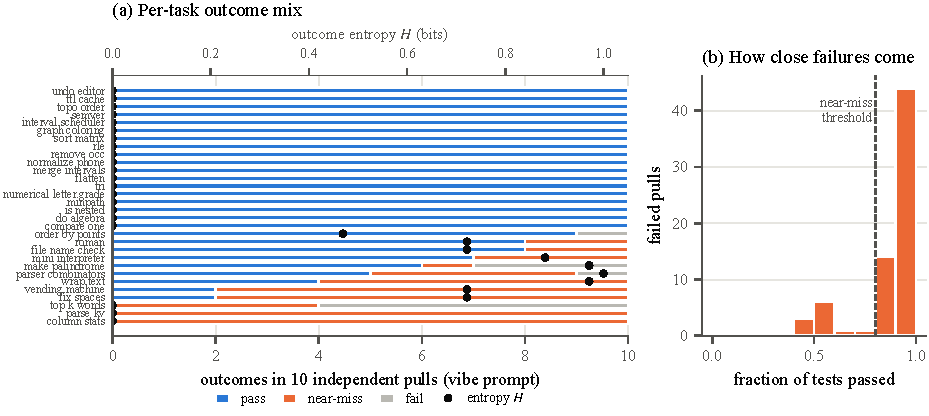
\includegraphics[width=0.92\linewidth]{../figures/fig1_variance_and_nearmiss.pdf}
\caption{Phase 1, vibe prompts, $N{=}10$ pulls per task. (a) Outcome mix per task (bars) and binary
outcome entropy (dots). (b) Fraction of tests passed by the \NFailedPulls{} failed pulls.}
\label{fig:baseline}
\end{figure*}
\subsection{Benchmark}
The suite has 10 algorithmic tasks adapted from HumanEval \citep{chen2021codex}
(e.g.\ \code{fix\_spaces}, \code{minPath}), 10 practical tasks in the style of MBPP
\citep{austin2021mbpp} (e.g.\ \code{parse\_kv}, \code{column\_stats}), and 10 original multi-function
or stateful tasks (an LRU cache with TTL, an integer interpreter with C-style division, a vending
machine with limited change, parser combinators, a dependency resolver that reports cycles, an undo/redo
editor, and others). Each task has a hidden reference solution and 8--10 tests, each pinning down one
rule. We verify that every reference passes its suite and that an empty module fails every test. Each
task has two prompts. The \emph{spec} prompt states every rule (\SpecWords{} words on average). The
\emph{vibe} prompt (\VibeWords{} words) names the API and the core intent and leaves edge cases
implicit, as in ``replace spaces with underscores, but if there are lots of consecutive spaces, replace
the whole run with a single \texttt{-}''; the hidden tests encode what the requester meant by ``lots'' (more
than two). The vibe condition is our primary setting.

\subsection{Harness}
Generations come from \Model{} via the Claude Code CLI (\code{claude -p}, version
\CliVersion) with no tools, settings or session persistence, a fixed system prompt asking for one code
block, and default sampling. Code runs in a fresh \code{python -I} subprocess with a scrubbed environment,
a 2\,s per-test timer and a 10\,s suite kill. Every call is logged with prompt, response, tokens, cost and
latency, and the log doubles as a cache keyed by (prompt, sample index), so conditions that request the
same draw receive the same sample (common random numbers).
The whole study used \NCalls{} calls (\TotalTokensM{}M tokens, \$\TotalCost{} at list prices).

\subsection{Retry Regimes}
In Regime A (\emph{blind pull}) each task is sampled $N{=}10$ times with an identical
prompt, as if the user pressed ``regenerate''. In Regime B (\emph{error-paste}) each blind pull seeds a
chain: if it fails, the pytest-style failure report (failing test, its assertion, got/expected values)
is pasted back with ``Please fix it.'' for up to five turns. All statistics are computed from the
logged attempts.

\subsection{Definitions}
Let attempt $a$ pass $s_a$ of $T$ tests. It is a \emph{pass} if $s_a{=}T$; a
\emph{near-miss} if the code loads and $s_a/T \ge 0.8$ or exactly one test fails; and a \emph{fail}
otherwise (including syntax errors and crashes on import). For task $i$ with empirical pass rate
$\hat p_i$ over $N$ pulls, outcome variance is $\hat p_i(1-\hat p_i)$ and outcome entropy is
\[H_i = -\hat p_i\log_2\hat p_i-(1-\hat p_i)\log_2(1-\hat p_i)\ \text{bits}.\] The near-miss rate is
$P(\text{near-miss}\mid\neg\text{pass})$. The marginal retry curve is the hazard
$h(t)=P(\text{pass at } t \mid \text{attempts } 1..t{-}1 \text{ failed})$. Blind pulls are i.i.d.\ within
a task, so we pool the plug-in estimate
\[h_A(t)=\frac{\sum_i(1-\hat p_i)^{t-1}\hat p_i}{\sum_i(1-\hat p_i)^{t-1}};\]
its decay reflects
selection (the sessions still failing are on harder tasks). For error-paste chains, $h_B(t)$ is the
empirical fraction of chains reaching turn $t$ that pass there. Confidence intervals resample tasks
(2{,}000 cluster-bootstrap replicates).

\subsection{Realistic Feedback (Phase 3)}
In Phases 1--2 every failure report comes from the complete
hidden suite and includes the expected values, the best case for pasting errors. Real programmers rarely
own tests that encode everything they meant. Phase 3 splits each suite: the programmer owns the first
\NVisible{} tests of each task (a rule fixed before any run; tests were ordered when the benchmark was
written), and all feedback in every condition comes from those. The \NHeldOut{} held-out tests only score
the final program. A session achieves \emph{intent pass} if its final program passes the full suite; it is a
\emph{silent failure} if the program passes every visible test but not the full suite, a loss disguised as a
win. The simulated programmer now privately holds the full specification but typed only the vibe prompt. A
\emph{vibecoder} pastes whatever their tests report and never volunteers detail; an \emph{attentive}
programmer reads each attempt and replies with one sentence of at most 40 words, an upper bound on what
engagement buys. Differences from the vibecoder are paired by task and bootstrapped over tasks.

\section{Baseline Results: Is Vibecoding a Slot Machine?}
\subsection{Payouts Are Intermittent and Failures Are Close}
Of \VibeN{} blind pulls, \VibePass{} passed
(\VibePassRate, 95\% CI \VibePassLo--\VibePassHi), \VibeNM{} were near-misses and \VibeFail{} failed
outright: \NmGivenFail{} of failures were near-misses (bootstrap CI \NmGivenFailLo--\NmGivenFailHi).
The median failure passed \MedianFracFailures{} of its tests (Fig.~\ref{fig:baseline}b). The payout
schedule is concentrated: \NAlwaysPass{} tasks passed every pull, \NNeverPass{} never passed, and
\NStochastic{} were genuinely stochastic, with mean entropy \StochEntropy{} bits among those (\MeanEntropy{}
bits over all 30). The original stateful tasks had the most stochastic tasks (\StochOriginal{} of 10).

\subsection{The Reels Spin but Land on the Same Symbols}
Independent pulls of the same prompt share only
\CodeSimilarity{} of their text on average (difflib ratio), so each regeneration looks new. Their
behaviour barely changes: ten pulls produced \DistinctBehaviours{} distinct pass/fail vectors per task,
and the most common failure signature accounts for \ModalSignatureShare{} of failed pulls (\code{fix\_spaces}
turned a double space into a dash in 8 of 10). These are consistent readings of an underspecified request,
which is why re-rolling rarely fixes them. The same tasks written as full specifications passed
\SpecN/\SpecN{} pulls (entropy \SpecEntropy): the randomness is the gap between what the user typed and what
their tests require.

\begin{figure*}[t]
\centering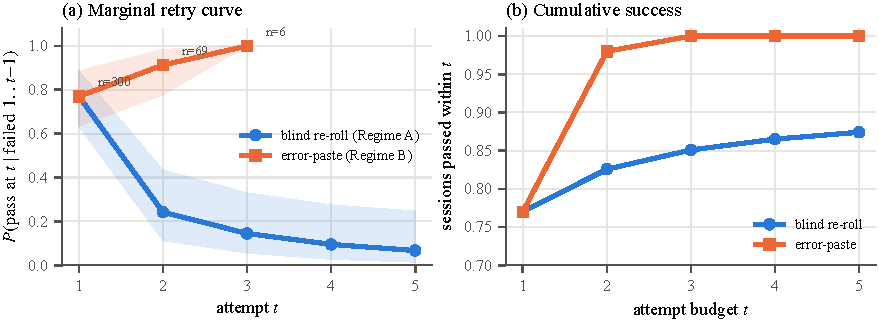
\includegraphics[width=0.9\linewidth]{../figures/fig2_retry_curves.pdf}
\caption{(a) Marginal retry curves with 95\% task-bootstrap bands; $n$ is the number of error-paste
chains reaching each turn. (b) Fraction of sessions passed within a budget of $t$ attempts.}
\label{fig:retry}
\end{figure*}

\subsection{Blind Retries Decay; Pasted Errors Converge}
The blind hazard falls from \BlindHazOne{} to
\BlindHazTwo{} on the second pull (CI \BlindHazTwoLo--\BlindHazTwoHi) and \BlindHazFive{} on the fifth;
five pulls lift cumulative success only from \BlindCumOne{} to \BlindCumFive{} (Fig.~\ref{fig:retry}).
Error-paste behaves differently: \EpHazTwo{} of the \EpReachedTwo{} chains that failed once passed on
the next turn, and all \EpReachedThree{} remaining chains passed on the third. Chains never regressed
(\RegressionRate{} of steps lost a test), consecutive attempts shared \ConsecSimilarity{} of their
text (edits, not re-rolls), and a near-miss was followed by a pass \PassAfterNM{} of the time versus
\PassAfterFail{} after a fail. The loop converges because the failure report contains the expected
values, which carry the intent the vibe prompt left out. All of that information comes from the test
suite; the programmer only carried it from the terminal to the chat. Our pre-registered budget rule
(stop where the next-attempt hazard falls below half that of the first retry, else the last observed turn)
gives $k^*{=}\KStar$ for every patch; on error-paste chains this is the default, since none reached a fourth turn.

\section{Designing and Evaluating ``Nicotine Patches''}
Each patch is a session protocol that controls what the programmer is shown and which decisions they
own. In Phase 2 all conditions observe the same vibe prompt and complete test feedback. Where a protocol
hands work to the programmer, a separately prompted model call stands in for them; its calls are excluded
from agent cost and its lines count as human-written. This proxy tests whether a protocol \emph{can} be
completed within its boundaries, not how people behave.

\subsection{Four Patches}
The first patch, P1 (\emph{retry budget with decomposition handoff}), runs error-paste for at most $k$ turns. On exhaustion
the agent must hand back a skeleton in which the decisions implicated by the failures live in 1--4
\emph{typed holes} (\code{hole\_*} functions with type hints, a docstring contract and body
\code{raise NotImplementedError}), plus 4--8 executable invariants over the public API. The programmer
fills the holes; a splice step keeps only their \code{hole\_*} code, enforcing the ownership boundary.

P2 (\emph{hidden best-of-5 with a behavioural diff}) tests five candidates privately, as in
sample-and-filter generation \citep{li2022alphacode}; only the best is shown, with a summary of which
tests the hidden candidates disagreed on. P3 (\emph{test-gated reveal with diagnosis}) shows code
only once it passes. A failing attempt is replaced by a diagnosis of at most two sentences without code,
phrased as a clarification the programmer adds to their request, close in spirit to test-driven intent
formalisation \citep{lahiri2022ticoder}.

In P4 (\emph{spec-first typed holes}), before any code exists the agent writes the API, the boilerplate and invariants, and leaves the core decisions as holes, following
the PL tradition of holes as partially specified program fragments \citep{solarlezama2008sketching,
omar2017hazelnut,omar2019livelit} and of properties as specifications \citep{claessen2000quickcheck};
retries iterate on the holes, never on the whole program. Each patch gets up to $k$ rounds.

\subsection{Agency Metrics}
A \emph{visible lottery outcome} is a complete model-written program shown together
with its score; under P3 the visible signal is ``withheld'' or a revealed pass. \emph{Visible entropy}
is the entropy (bits) of the visible signals per task, averaged over tasks. \emph{Passive retries}
are regenerations that add no human information. \emph{Decision points} are holes to fill or
clarifications to accept. \emph{Human lines} is the share of the final program written inside
human-owned holes. \emph{Spec soundness} is the share of model-written invariants that hold on the
hidden reference.

\begin{table*}[t]
\centering\small\setlength{\tabcolsep}{3.6pt}
\caption{Phase 2, complete feedback; 10 sessions per task (P4: 5), $k{=}\KStar$ unless noted. H: visible
entropy (bits); NM: visible near-misses; Ret.: passive retries; Dec.: decision points; Hum.: human-written
share of final lines; Sound: invariants holding on the reference; agent calls, kTokens and latency (s).
All per session.}
\label{tab:patches}
% Generated by analysis/report_numbers.py. Do not edit.
\begin{tabular}{@{}lrrrrrrrrrr@{}}
\toprule
Condition & Pass & H & NM & Ret. & Dec. & Hum. & Sound & Calls & kTok & Lat. \\
\midrule
Slot machine (baseline) & 100\% & 0.38 & 0.21 & 0.25 & 0.00 & 0\% & -- & 1.2 & 2.9 & 7.0 \\
\addlinespace[2pt]
P1 retry budget, $k{=}1$ & 98\% & 0.29 & 0.19 & 0.00 & 0.41 & 7\% & 93\% & 1.2 & 3.3 & 8.8 \\
P1 retry budget, $k{=}2$ & 99\% & 0.39 & 0.21 & 0.23 & 0.05 & 1\% & 92\% & 1.2 & 2.9 & 7.1 \\
P1 retry budget, $k{=}3$ & 100\% & 0.38 & 0.21 & 0.25 & 0.00 & 0\% & -- & 1.2 & 2.9 & 7.0 \\
\addlinespace[2pt]
P2 hidden best-of-5 & 100\% & 0.16 & 0.11 & 0.11 & 0.00 & 0\% & -- & 5.6 & 12.0 & 7.2 \\
P3 test-gated reveal & 99\% & 0.34 & 0.00 & 0.00 & 0.30 & 0\% & -- & 1.6 & 3.6 & 8.7 \\
P4 typed holes & 85\% & 0.00 & 0.00 & 0.00 & 2.19 & 31\% & 92\% & 1.0 & 4.8 & 14.9 \\
\bottomrule
\end{tabular}

\end{table*}

\begin{figure*}[t]
\centering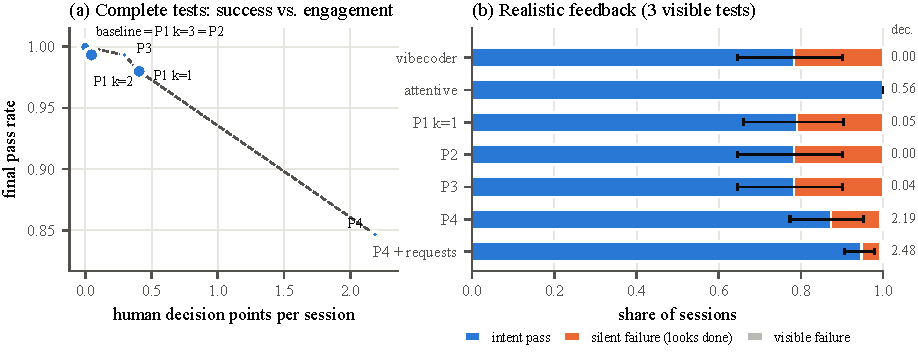
\includegraphics[width=0.9\linewidth]{../figures/fig3_patch_tradeoffs.pdf}
\caption{(a) Complete feedback: final pass rate against decision points per session (dashed: Pareto front;
marker area: visible near-misses). (b) Realistic feedback: how sessions end, with 95\% task-bootstrap CIs on
intent pass and decision points per session at right.}
\label{fig:tradeoffs}
\end{figure*}

\subsection{Results with Complete Feedback}
The baseline reaches \BasePass{} but shows \BaseNM{} near-misses and
\BaseRetries{} passive retries per session, and the programmer decides nothing (Table~\ref{tab:patches}).
P1 at $k{=}\KStar$ never triggers, because no chain needed a fourth attempt; a budget pays off only
when it binds. At $k{=}1$ the handoff fired \POneKOneHandoffs{} times and \POneKOneRescue{} of handoffs ended in
passing code, for \POneKOnePass{} overall with \POneKOneDecisions{} decisions per session. P2 cuts
visible near-misses by \PTwoNMRed{} at \PTwoTokX$\times$ the tokens, and the programmer still decides nothing.
P3 shows no near-misses, passes \PThreePass{} at \PThreeTokX$\times$ the tokens, and \PThreeCodeFree{} of
its \PThreeNHints{} diagnoses passed an automatic code detector (the rest quote example inputs, not
implementations). P4 also shows no lottery outcomes and gives the programmer \PFourDecisions{} decisions
and \PFourHumanFrac{} of final lines; \PFourSoundness{} of its \PFourInvTotal{} invariants hold on the reference.
It passes only \PFourPass{} (\PFourPassOriginal{} on stateful tasks): \PFourSingleFail{} of its \PFourFailures{}
failures end one test short because the skeleton fixed the deciding rule in boilerplate, e.g.\ whether inserted
coins can be returned as change. On the \NContested{} contested tasks the baseline still passes
\BaseContestedPass{} but shows \BaseContestedNM{} near-misses per session. No patch can beat it on success here,
because the failure report already hands the model the intent. Phase~3 removes that advantage.

\section{Realistic Feedback: Does the Baseline Still Win?}
\begin{table*}[t]
\centering\small\setlength{\tabcolsep}{3.4pt}
\caption{Phase 3, realistic feedback (\NVisible{} visible tests per task). $\Delta$: points vs.\ the vibecoder,
paired by task. Silent: passes every visible test, not the full suite. Turns: programmer actions per session.}
\label{tab:realistic}
% Generated by analysis/report_numbers.py. Do not edit.
\begin{tabular}{@{}lrrrrrrr@{}}
\toprule
Condition & Intent pass [95\% CI] & $\Delta$ pts [95\% CI] & Silent & NM & Dec. & Turns & kTok \\
\midrule
Vibecoder (paste errors) & 78\% [65\%, 90\%] & -- & 22\% & 0.01 & 0.00 & 0.03 & 2.2 \\
Attentive programmer & 100\% [100\%, 100\%] & $+$22 [$+$10, $+$35] & 0\% & 0.01 & 0.56 & 1.56 & 3.7 \\
\addlinespace[2pt]
P1 retry budget, $k{=}1$ & 79\% [66\%, 90\%] & $+$1 [0, $+$2] & 21\% & 0.01 & 0.05 & 0.07 & 2.3 \\
P2 hidden best-of-5 & 78\% [65\%, 90\%] & 0 [0, 0] & 22\% & 0.00 & 0.00 & 0.01 & 10.8 \\
P3 test-gated reveal & 78\% [65\%, 90\%] & 0 [0, 0] & 22\% & 0.00 & 0.04 & 0.04 & 2.3 \\
P4 typed holes & 87\% [77\%, 95\%] & $+$9 [$-$3, $+$22] & 12\% & 0.00 & 2.19 & 1.03 & 4.8 \\
P4 + hole requests & 95\% [91\%, 98\%] & $+$16 [$+$5, $+$30] & 5\% & 0.00 & 2.48 & 1.19 & 5.9 \\
\bottomrule
\end{tabular}

\end{table*}

\subsection{The Baseline's Perfect Score Was an Artifact}
With only their own tests, the
vibecoder ends every session believing the code works (\RVibeVisPass{} pass their visible tests), but only
\RVibePass{} pass the full suite (CI \RVibePassLo--\RVibePassHi). \RVibeSilent{} of sessions are silent
failures, spread over \RSilentTasks{} tasks; on the \NContested{} contested tasks (those with a failed
Phase~1 pull) the vibecoder is right \RVibeContestedPass{} of the time. The near-miss has not gone away; it
has become invisible, which is the coding analogue of a loss disguised as a win \citep{dixon2010ldw}. A
programmer who reads each attempt and states what they meant closes the gap: the attentive condition
reaches \RAttPass{} (\RAttDelta{} points, CI \RAttDeltaLo{} to \RAttDeltaHi) with \RAttClar{} clarifications per
session of \RAttClarWords{} words on average, and accepts the first attempt in \RAttAcceptFirst{} of sessions.

\subsection{Failure-Triggered Patches Inherit the Blind Spot}
P1, P2 and P3 act only when a test fails, and the
programmer's tests flagged \RVisFailFirst{} of 300 first attempts: P1's handoff fired \ROneHandoffs{} times, P2
ranks candidates by tests they all pass (at \RTwoTokX$\times$ the tokens), and P3 reveals code once the visible
tests pass. Their intent-pass rates (\ROnePass, \RTwoPass, \RThreePass) match the vibecoder's.

\subsection{Asking Before Generating Helps}
P4 asks for the core
decisions before any code exists, so the programmer's intent reaches the program whether or not a test fails.
Plain P4 reaches \RFourPass{} (\RFourDelta{} points, CI \RFourDeltaLo{} to \RFourDeltaHi), a gain whose interval
includes zero: as in Phase~2, skeletons sometimes fix the deciding rule outside every hole (\RFourSilent{}
silent failures; \RFourPassOriginal{} on stateful tasks). With hole requests the programmer can name such a
decision and the agent re-scaffolds once. \RFourPlusRequests{} of 150 sessions used a request and
\RFourPlusRequestPass{} of those passed. P4 with hole requests reaches \RFourPlusPass{} (\RFourPlusDelta{} points,
CI \RFourPlusDeltaLo{} to \RFourPlusDeltaHi; \RFourPlusVsFour{} over plain P4, CI \RFourPlusVsFourLo{} to
\RFourPlusVsFourHi) and \RFourPlusPassOriginal{} on stateful tasks, with \RFourPlusDecisions{} decisions per
session at \RFourPlusTokX$\times$ the vibecoder's tokens. It is the only patch whose gain excludes zero, and it
recovers most of the attentive programmer's gain by asking for decisions rather than a review of every attempt.

\subsection{Discussion}
With realistic tests the slot machine gets worse: the programmer sees a win, ships it,
and is sometimes wrong. Interventions that change how failures look (P1--P3) need a test to fail; those that
ask for decisions up front do not. What the human is handed should be checkable against what they meant: a
hole with a contract, an invariant that runs, a clarification. P3's diagnoses still help when tests fail, but
some are fluent and wrong (two for \code{parser\_combinators} reversed the intended semantics).

\section{Limitations and Future Work}
We study one model (\Model) on 30 Python tasks, and hidden tests define intent. The tasks, tests, reference
solutions and vibe prompts were written by an AI assistant for this study rather than collected from
programmers, and the vibe prompts were written after a pilot showed that full specifications passed every
pull; we report both conditions rather than tune either. The programmer is a model in Phases 2 and 3, so
pass rates show that a protocol \emph{can} be completed within its boundaries, not that people will complete
it. Phase 3 assumes a programmer who knows what they mean and says it only when asked; that is the definition
of vibecoding, but it is an assumption, and the attentive programmer sometimes quotes a short snippet. The
first-three-tests rule is one choice; others would move the numbers. Agency metrics are structural counts,
not comprehension. A splice bug in our first P1/P4 run was fixed and those conditions re-run (first run
archived under \code{results/phase2/superseded/}).

The most important next step is a user study ($N{\approx}24$; baseline, P3, P4, P4 with hole requests) that
measures silent failures, time to pass, comprehension and the urge to regenerate. Real vibe prompts collected
from programmers, and a sweep that adds missing details to the prompt one at a time, would test how far the
specification gap explains the variance.

\section{Conclusion}
Under underspecified requests, a coding agent pays out intermittently and its losses look
like wins. With complete tests, pasting errors closes the gap without involving the programmer; with the
programmer's own few tests, \RVibeSilent{} of sessions ship wrong code that looks finished. Interventions that
only change how failures look cannot fix what the tests do not catch. Typed holes that ask the programmer for
decisions before generation, and let them reopen decisions the scaffold made, recover most of the lost
accuracy and give the programmer real work. The
useful fix for the slot machine is not more pulls but a better specification, drawn from the person who has it.

{\small
\section*{Code and Data}
The benchmark, harness, analysis scripts, every logged model call and the replayable demos are available at
\\\url{https://github.com/leebr27/vibecoding-slotmachine-final}.

\section*{AI Disclosure}
The benchmark (tasks, tests, reference solutions, vibe prompts), the harness, the
analysis and a draft of this report were produced with an AI coding assistant (Claude Code). Every number
is generated from the logged runs by \code{analysis/report\_numbers.py}.
}

{\scriptsize
\bibliographystyle{abbrvnat}
\bibliography{refs}
}
\end{document}
